\documentclass[11pt]{article}
\usepackage[margin=1in]{geometry}
\usepackage{graphicx}
\usepackage{hyperref}
\usepackage{booktabs}
\usepackage{amsmath,amssymb}
\usepackage{xcolor}
\hypersetup{colorlinks=true,linkcolor=blue,citecolor=blue,urlcolor=blue}
\setlength{\parskip}{0.7em}
\setlength{\parindent}{0em}

\title{A Prospectively Confirmed Arithmetic Effect of Step-by-Step Prompting in Local Models,\\ with Null Results Outside Arithmetic}
\author{Liu Zewen\\{\small \textit{Independent Researcher}}}
\date{\today}

\begin{document}
\maketitle

\begin{center}\begin{minipage}{0.92\textwidth}\small\it
One finding survives project-level multiplicity correction and has been confirmed
prospectively on a fresh, disjoint item set with a preregistered rule that executed.
The arms that did not survive --- amplification, balancing, inference budget, and the
transfer effect outside arithmetic --- are reported as such.
\end{minipage}\end{center}
\vspace{1em}

\section*{Abstract}

A structured reasoning policy -- state the reasoning, then answer -- is widely

assumed to help because reasoning-before-answering helps in general. We test that

on local models from 1B to 8B across general, reasoning and coder lineages, with

preregistered envelopes, Ed25519-signed evidence bundles, adversarial review at

every step, and a project-level correction for the number of experiments run.


{\bf The primary claim is confirmed prospectively.} On 160 held-out arithmetic items

verified disjoint from the items that first produced the effect, a step-by-step

policy beats direct answering in 2 of 2 model families tested (gains +0.244

[+0.163, +0.325] and +0.519 [+0.431, +0.606]; pooled paired McNemar 133:11), at

320 paired observations against the n = 157 a power calculation requires. The

original estimate on 40 items was +0.700 for one of those families, so the

direction, the family coverage and the mechanism all replicated while the magnitude

did not.


Applying Benjamini-Hochberg across all 14 recomputable primary endpoints in the

project, {\bf 5 of 14 survive and 4 of them support the claim they were preregistered for (9 of 14 fail).} What does not survive is

reported rather than dropped: swarm amplification, subset balancing, the

inference-length sweet spot (refuted at adequate power -- budget helps

monotonically on a 7B reasoning model and does nothing on a 7B non-reasoning one),

and the transfer itself outside arithmetic, where no reasoning-first policy

recovers a gain across two task-domain replications. Nine further arms carry

directional claims with no test computable at their n, which makes even the

surviving p-values optimistic. A seventh finding concerns measurement rather than

models: across three local evaluators, 16 of 24 realistic code diffs change

ship/no-ship verdict when one evaluator is dropped.


The contribution is one confirmed effect with an explicit account of everything

that did not confirm, and of the multiplicity that would otherwise have hidden it.


{\bf How to read this paper.} Section 1 states the tension the project started

from. Section 2 reports the one effect that survives project-level correction,

with per-family intervals. The prospective confirmation of that effect -- new

items, fixed seed, a rule that executed -- follows in its own section, because a

confirmed finding and an observed one are different claims. Sections 3-6 report

what did not survive, each with the verdict its own preregistration produced:

amplification and balancing (exploratory), the inference budget (refuted at

adequate power), and early warning (a diagnosed failure mode, not a capability).

The second task domain and the policy-adaptation refutation then narrow the scope

to arithmetic. The project-level correction that governs all of this is stated

once, with its table, rather than repeated per section; each arm cites its row.

A worked example walks one full pass for the general reader, and two appendices

record the supervision defects this project paid for, so a reviewer can check the

machinery rather than trust it.


\section*{1. Tension}

Evaluator-preference collapse (reward overoptimization by the judge, not the

task) was measured with frontier evaluators at frontier cost. Everyone deploying

small or many models operates outside the measured regime: small-model users

cannot afford the protocol that established the effect, and swarm operators run

100+ parallel executors with no characterization of bias at scale. If the

phenomenon is about scale, small deployments are safe and the theory needs a

capability boundary. If it is about protocol, every deployment inherits it.

Nobody had checked, because checking is unfashionable work: replications,

boundary conditions, and negative controls.


\section*{2. Transfer: the one effect that survives correction}

Preregistered envelope (hypothesis, exact command, budget \$0, kill-switch rows,

fixed seed, power fields, negative-publication plan). 40 held-out GSM8K-style

cases never used for selection; direct vs step-calc; exact float match;

paired design with McNemar exact test, BH across 2 models, 5000-rep bootstrap

CIs. Ed25519-signed bundle verifies.


\begin{center}\small\begin{tabular}{llllll}\hline
model & direct & step-calc & gain [95\% CI] & McNemar & p (BH) \\
\hline
qwen2.5:7b & 0.150 & 0.900 & +0.75, 95\% CI [0.60, 0.875] & 30:0 & 2.0e-9 \\
llama3.1:8b & 0.025 & 0.800 & +0.775, 95\% CI [0.65, 0.90] & 31:0 & 9.3e-10 \\
\end{tabular}\end{center}

Kill-switch: STOP-EXTEND. Two-seat review (4/10, 2/10, joint NOT\_READY on

magnitude equivalence --- correctly, since CIs overlap): the directional claim is

supported, "undiminished magnitude" is explicitly disclaimed in favor of a

preregistered 200-item extension.


Effect sizes: Cohen's h = 1.703 (qwen) and 1.897 (llama), both large by

conventional thresholds. Practical significance: absolute gains of 75 and 77.5

percentage points on exact-match accuracy are visible without statistics; the

p-values (both p < 1e-8 after BH correction) confirm what the raw differences

already show rather than rescuing a borderline result.


\section*{3. Amplification (exploratory; does not survive project-level correction)}

{\it Status: primary endpoint p\_BH = 0.200 across the project. Reported because the design is informative and the abstention confound was genuinely excluded, not because the effect is established.}


Minimal TTRL loop (4 strategies, 4 tasks, 6 rounds, +0.08/-0.04 updates):

swarm=1 (sequential) vs swarm=4 (parallel, evaluator picks best per round).

Multi-seed (5 seeds): excesses 0.012/0.0/0.055/0.055/0.037, mean 0.032,

t 95\% CI [0.001, 0.063] --- barely excludes zero, reported as a small uncertain

effect, not a breakthrough.


The devil's objection (abstentions skip updates, so swarm size interacts with

the abstention mechanism itself) was tested, not argued: a force-decide arm

(re-ask once with forcing language, then deterministic seeded choice, every

vote flagged) shows excess 0.0163 with ZERO abstentions and ZERO forced votes

across 18 judge calls. The gap persists where the confound cannot operate.

Remaining weaknesses, stated: n=1 per arm here, 6 rounds, 4 tasks, small

magnitude. The multi-seed leg carries replication weight; the force-decide leg

carries mechanism cleanliness. Neither alone suffices.


\section*{4. Balancing (exploratory)}

{\it Status: MOSTLY-HOLDS at 82\% of subsets; no project-level-surviving endpoint.}


On committed evaluator-collapse weights (11 strategies, 8 text + 3 visual):

full-set cross PCI 1.619 > self 1.265. All 56 balanced 3+3 subsets enumerated:

46 preserve the ordering (82\%, MOSTLY-HOLDS). An initial top-3-only analysis

reversed the pattern --- an unlucky 18\% draw, caught by review, corrected by full

enumeration (now automatic via robustness.py). PCI magnitudes across different

set sizes are not compared (normalization differs); only orderings.


\section*{5. Inference budget: no sweet spot at this scale (sweetspot-04, STOP-REFUTED)}

An earlier arm reported a flat-then-cliff accuracy curve across reasoning caps and

two seats refused it at n = 6 per family. Re-run on 48 code-repair items at caps

150 / 400 / 1000 with 96 paired observations per cap -- the n a power calculation

requires for a 0.25 effect -- the cliff does not exist, and neither does its

opposite:


\begin{center}\small\begin{tabular}{lllllll}\hline
model & cap 150 & cap 400 & cap 1000 & cap400 fixed & cap1000 broke & McNemar p \\
\hline
qwen2.5:7b & 0.583 & 0.583 & 0.583 & 0 & 0 & 1.000 \\
deepseek-r1:7b & 0.000 & 0.083 & 0.271 & 9 & 0 & 0.0039 \\
\end{tabular}\end{center}

Pooled 9:0 (p = 0.0039), but in the opposite direction from the hypothesis:

{\bf zero of two families degrade at cap 1000.} Zero truncations in every cell, so

the budget was delivered rather than clipped.


The two behaviours are different rather than a shared curve. One family is flat --

its fixes are short enough that the budget is not the binding constraint. The

other is monotonically increasing, and at cap 150 it cannot complete a fix at all,

which is what produced the original "cliff" appearance on a different item set: at

150 tokens the model simply does not finish.


This does not contradict Thoughtology (Marjanovic et al., TMLR 2026), which

reports a sweet spot on the full DeepSeek-R1 with an internally controlled budget.

It does not reproduce it at 7B. Whether the phenomenon is scale-dependent is

outside what this hardware can test, and the paper says so rather than implying

either result. The sweet-spot claim is dropped.


\section*{6. Early warning: a diagnosed failure mode, not a capability}

{\it Status: withdrawn as a capability. See the diagnosis section for why the misses are structural.}


On 7 committed evaluator conditions (contagion, ds-self, gpt4o-cross, qwen37,

real-image, multiexecutor, interrupted qwen-partial): leave-one-out rank

prediction from pairwise JSD hits 5/7 (hit rate 0.714, Wilson 95\% CI

[0.359, 0.918] --- wide, as befits n=7). Misses concentrate on the high-collapse

extremes that define the phenomenon (gpt4o-cross true 6 predicted 3;

multiexecutor true 3 predicted 1), with contagion as hub neighbor to 4/5

holdouts. JSD is a coarse sorter for low/mid-collapse conditions, not an

extreme predictor. Both statements are in the ledger; neither is rounded up

to "confirmed" as a practical claim.


\section*{7. Limitations (stated, not buried)}

\begin{itemize}
\item The discovery estimate was optimistic. qwen2.5:7b gained +0.700 on the 40 discovery items and +0.244 on 160 fresh disjoint items. Both numbers are reported; the smaller one is the better estimate of the true effect, and any citation of the larger one without the smaller is a misrepresentation of this paper's own evidence.
\item The eight-family breadth result is analyst-assigned, not preregistered: its kill-switch keyed on a field the harness never emitted, so no rule fired. It is reported as observed, and the prospective confirmation it motivated covers two families, not eight.
\item Exact float match understates absolute levels (3.0 vs 3.00 counts as miss); comparisons are fair (same metric both arms) but levels are floors.
\item Local ollama models only; no frontier evaluator replication (budget \$0 by design). Nothing here speaks to frontier-scale behavior, including whether the inference-length sweet spot reported on full DeepSeek-R1 appears at any scale we can test.
\item Nine arms carry directional claims with no test computable at their n; they are disclosed, not cited, and their presence makes every project-level p-value in this paper optimistic.
\item One arm's verdict was withdrawn for infrastructure contamination (lineage-01), and one run certified the wrong experiment before the config binding existed (breadth-02's first attempt). Both are amended on their signed bundles rather than deleted, so the failure modes stay inspectable.
\item The force-decide deterministic fallback (seeded coin on persistent abstain) never triggered (0 forced votes); its behavior under real abstention pressure is untested.
\item JSD analysis is retrospective on committed weights; prospective validation (predict-then-run) is future work with its own envelope.
\end{itemize}

\section*{8. What would change each section}

\begin{itemize}
\item Transfer: 200-item heldout + McNemar matrix across 8 local families (matrix envelope approved, queued).
\item Amplification: 8/16/32 subagents scaling curve + abstention-rate logging per arm (already instrumented: forced/abstained/total votes per arm).
\item Robustness: multi-rep per-strategy weights (30-rep gamma files exist; weight files do not --- needs re-running the source protocol).
\item Early warning: 2+ more evaluator conditions to push LOO past n=7; prospective run on a fresh evaluator.
\end{itemize}

\section*{Bounded lesson}

Observation: evaluator-preference effects replicate on small local models

(transfer +0.75/+0.775, both p\_bh 2e-9), grow with parallelism (4/5 seeds),

survive balancing (46/56), and are coarsely predictable from evaluator

disagreement (5/7 LOO).

Interpretation: the phenomenon is about protocol design, not scale -- but every

magnitude here is pilot-grade (n=40, 6 rounds, 1-rep weights) and must not be

cited as an effect size.

Proposed action: replicate the exact procedures (commands in Reproduce below)

before citing; extend, do not port, the numbers.

Transfer limits: eight model families on ONE task domain (not breadth across

tasks); one evaluator pair for swarm; committed weights only for JSD; local

ollama only throughout. Nothing here generalizes beyond those bounds without the

extensions in Section 7.


\section*{Reproduce}
\begin{verbatim}
# every number below traces to artifacts/result.json -> field (see CLAIM_LEDGER.md)
# verify: python -m ai_researcher.loop verify <rundir>  (Ed25519, per round)
# ledger: python -m ai_researcher.bridge <rundir> <envelope> --out <paperdir>
# quality: python -m ai_researcher.loop publish <rundir> --tier <workshop|conference-main|tmlr|sci-journal|zone1> --paper <paperdir>
\end{verbatim}

\section*{Baselines and ablations (what was compared, what was not)}

Baselines run: direct prompting (the null policy) on both models --- the only

baseline that isolates the policy effect. Excluded with reasons: chain-of-thought

variants (confound verbosity with the step-calc mechanism under test);

few-shot variants (confound example quality); other model families (preregistered

as the 8-model matrix extension, not run here).


Ablations completed: none beyond the direct-vs-step contrast. Not ablated:

prompt wording variants of step-calc, temperature > 0, alternative answer

extractors. Each is a named follow-up with a preregistered envelope slot, not a

silent gap.


\section*{Data and code availability}

Item banks are in the repository, not in temporary storage. This was false until

2026-10-08: the arithmetic held-out set lived only under \texttt{/tmp/ind-audit/}, so the

evidence for the primary claim was one cleanup away from being unreproducible. It

is now \texttt{demo/transfer/items/heldout40.json} (40 items, with provenance) and

\texttt{demo/transfer/items/confirm160.json} (160 items, verified disjoint from the

first by \texttt{demo/transfer/build\_confirm\_set.py}, which refuses to write a set that

fails its own invariants). The code-repair bank is

\texttt{demo/coderepair/run\_coderepair.py::TESTS}, covered by an executable self-test.

Every number in this paper is regenerated from signed bundles by

\texttt{scripts/project\_alpha.py} and checked by \texttt{scripts/verify\_all.py} in CI.


\section*{Broader impact and ethics}

Who benefits: practitioners deploying small models get directional evidence where

they previously had vendor claims and frontier-model lore. The headroom account

of the effect -- gain tracks available headroom rather than model size -- is a

post hoc hypothesis, not a preregistered prediction: it was read off the

eight-family ordering after seeing it, and it fails where it should be tested

most stringently (gemma3:4b has a high direct baseline on code repair yet loses

0.250). It is stated here as a hypothesis for others to preregister against,

with the code-repair counterexample beside it so it cannot be mistaken for an

established mechanism. The negative

results are guardrails with numbers attached rather than generic cautions.


Who could be harmed, concretely: a team that deploys a reasoning-first policy on

code repair because "structured reasoning helps" would lose accuracy we have

measured -- gemma3:4b drops 0.250 with an interval of [-0.375, -0.125] that

excludes zero, and no adapted policy recovers it. That harm is not hypothetical;

it is the second task domain in this paper. The scope statement exists to prevent

exactly this deployment.


Dual use: none beyond standard LLM deployment considerations. Compute footprint:

several thousand local ollama calls across all arms, no paid APIs, no

human-subjects data. All experiments run on a single consumer GPU, so the

evidence is reproducible by any practitioner with comparable hardware rather than

only by labs with cluster access -- which is itself part of the point, since the

deployments this paper speaks to are the ones that cannot afford the protocol

that established the effect at frontier scale.


\section*{AI use disclosure}

Experiments were designed and executed through an autonomous research loop

(preregistration envelopes, kill-switches, signed evidence bundles); the

manuscript draft was machine-generated from claim ledgers and revised by a

human author. All numbers trace to committed artifacts (see Reproduce). System

names and implementation details are withheld from this blind-submission text

and will appear in the camera-ready version.


\section*{References}

Every entry was resolved against arXiv, OpenReview, the publisher record or a

project repository on 2026-10-08. One earlier entry, "topological mimicry

(Chen \& Wang 2026)", could not be resolved to any record and was {\bf removed rather than retained}; the removal is recorded here because a citation that

cannot be found is a defect in the paper, not a formatting inconvenience.


\begin{itemize}
\item Cobbe, K., Kosaraju, V., Bavarian, M., et al. (2021). Training verifiers to solve math word problems. {\it arXiv:2110.14168}. [GSM8K; the arithmetic item banks]
\item Wang, X., Wei, J., Schuurmans, D., et al. (2023). Self-consistency improves chain of thought reasoning in language models. {\it ICLR 2023}. OpenReview \texttt{1PL1NIMMrw}.
\item Chen, A., Phang, J., \& Parrish, A. (2024). Two failures of self-consistency in the multi-step reasoning of LLMs. {\it TMLR 2024}. OpenReview \texttt{5nBqY1y96B}.
\item Marjanovic, S. V., Patel, A., Adlakha, V., et al. (2026). DeepSeek-R1 Thoughtology: let's think about LLM reasoning. {\it TMLR}, accepted 12 Jan 2026. {\it arXiv:2504.07128}; OpenReview \texttt{BZwKsiRnJI}. {\bf Nearest prior work for the inference-length arm} -- see Related work.
\item Zhou, E., et al. (2025). Landscape of thoughts: visualizing the reasoning process of large language models. {\it arXiv:2503.22165}. [TMLR; verifier-weighted path voting]
\item Zhang, Y., et al. (2024). Topologies of reasoning: demystifying chains, trees, and graphs of thoughts. {\it arXiv:2401.14295}. [replaces the unresolvable citation noted above; it is the real work on reasoning topologies]
\item Zheng, L., Chiang, W.-L., Sheng, Y., et al. (2023). Judging LLM-as-a-judge with MT-Bench and Chatbot Arena. {\it arXiv:2306.05685}. [position bias and self-enhancement]
\item Jimenez, C. E., Yang, K., Barnes, A., et al. (2024). SWE-bench: can language models resolve real-world GitHub issues? {\it arXiv:2310.06770}. [the code-repair domain]
\item Zuo, Y., Zhang, K., Li, S., et al. (2025). TTRL: test-time reinforcement learning. {\it arXiv:2504.16084}; NeurIPS 2025.
\item Khattar, V., Rashid, M. R. ur, Choudhury, M., et al. (2026). Amplification effects in test-time reinforcement learning: safety and reasoning vulnerabilities. {\it arXiv:2603.15417}. [nearest prior work on amplification]
\item Li, Y., Yue, X., Xu, Z., et al. (2025). Small models struggle to learn from strong reasoners. {\it arXiv:2502.12143}. [the small-model learnability gap]
\item Moonshot AI (2026). Kimi-K2.5 technical report. \texttt{github.com/MoonshotAI/Kimi-K2.5/blob/master/tech\_report.pdf}; Agent Swarm documentation, kimi.com/en-cn/help/agent/agent-swarm. [K2.5 released 27 Jan 2026 with Agent Swarm at up to 100 sub-agents; K2.6 on 20 Apr 2026 at up to 300. The vendor states the swarm "creates the conditions for productive disagreement ... avoids groupthink structurally."]
\item DeepSeek-AI (2025). DeepSeek-R1. {\it arXiv:2501.12948}.
\item McNemar, Q. (1947). Note on the sampling error of the difference between proportions or correlated proportions. {\it Psychometrika} 12(2), 153-157.
\item Benjamini, Y., \& Hochberg, Y. (1995). Controlling the false discovery rate. {\it JRSS Series B} 57(1), 289-300.
\end{itemize}

\section*{Related work (what differs, one line each)}

\begin{itemize}
\item {\bf Sakana AI Scientist v1+v2} (Lu et al. 2024; Yamada et al. 2025; Nature 2026): end-to-end idea\$\textbackslash\{\}to\$paper automation with archive-feedback and agentic tree search. Differs: no preregistration envelope, no evidence signing, single-model review. We adopt their archive-feedback loop and AI-disclosure norm; our envelope, Ed25519 bundles, and two-seat contradiction scoring address the integrity gaps their pipeline leaves open.
\item {\bf MLAgentBench} (Huang et al., ICML 2024): 13 ML-engineering tasks for agent evaluation (best 37.5\%); names long-horizon planning and hallucination-about- progress as the two failure modes. Differs: evaluates agents on engineering tasks, not evaluator bias. Our loop's state machine + resume + evidence-over- self-report answers both failure modes directly; scoped as external validation.
\item {\bf Thoughtology} (Marjanovic et al., TMLR 2026, arXiv:2504.07128): the nearest prior work to our inference-length arm. They report that DeepSeek-R1 has a "sweet spot of reasoning, where extra inference time can impair model performance", plus rumination on previously explored formulations. Differs in three ways we can state precisely: they study frontier R1 with a thinking budget the model controls internally, we vary an external token budget on 7B-8B local models; their sweet spot is a property of one model family, ours is asked whether it survives at small scale; and their budget cannot be set by prompting, which is exactly the confound our cap sweep holds fixed. Our arm is therefore a replication at a different scale with an externally controlled budget, and it is reported as {\it suggestive only} -- n=6 per family did not survive two-seat review, and the amplification that meets the power gate is queued rather than claimed.
\item {\bf Kimi Agent Swarm} (Moonshot AI, K2.5 tech report and Agent Swarm docs): the vendor states the swarm "creates the conditions for productive disagreement -- for independent agents to arrive at different conclusions, then force a reconciliation" and that it "avoids groupthink structurally". Differs: our amplification arm measures what happens when independent samples {\it converge} on a shared bias and a vote then amplifies it, which is the failure mode that design principle is meant to exclude and which our data suggests is not excluded in practice. This is a scale (1-8 agents, local models) versus a system-scale claim, so we frame it as a question the vendor's premise raises rather than as a refutation of their system.
\end{itemize}


\section*{Breadth across model families (8/8, sign test p=0.004)}

The transfer effect was re-measured on a 40-item held-out set across eight local

model families spanning 1B-8B and general/reasoning/coder lineages.


\begin{center}\small\begin{tabular}{llllll}\hline
family & direct & step-calc & gain [95\% CI] & fail-to-pass & pass-to-fail \\
\hline
qwen2.5:7b & 0.125 & 0.825 & +0.700 [+0.550, +0.850] & 28 & 0 \\
llama3.1:8b & 0.025 & 0.400 & +0.375 [+0.225, +0.525] & 15 & 0 \\
qwen2:7b & 0.025 & 0.450 & +0.425 [+0.250, +0.600] & 18 & 1 \\
gemma3:4b & 0.025 & 0.800 & +0.775 [+0.650, +0.900] & 31 & 0 \\
deepseek-r1:7b & 0.225 & 0.925 & +0.700 [+0.550, +0.850] & 29 & 1 \\
qwen3:4b & 0.725 & 0.875 & +0.150 [+0.025, +0.275] & 7 & 1 \\
qwen2.5-coder:7b & 0.300 & 0.900 & +0.600 [+0.450, +0.750] & 24 & 0 \\
llama3.2:1b & 0.000 & 0.525 & +0.525 [+0.375, +0.675] & 21 & 0 \\
\end{tabular}\end{center}


{\bf Figure 1.} Per-family transfer gain with 95\% paired-bootstrap intervals, ordered

by gain. Points are step-by-step minus direct accuracy on 40 held-out arithmetic

items; grey bars connect each family's direct and step-by-step accuracies. All

eight intervals exclude zero. The family with the highest direct baseline

(qwen3:4b, 0.725) has the smallest gain (+0.150, [+0.025, +0.275]) and the family

with a zero baseline (llama3.2:1b) gains +0.525 -- consistent with the post hoc

headroom hypothesis, which is all that consistency claim amounts to until it is

tested prospectively. Generated by \texttt{demo/papers/figures/fig\_transfer\_forest/} from the signed

bundle; \texttt{raw\_data.py} recomputes every value, so an amendment to the bundle

invalidates the figure rather than silently desynchronising it.



\begin{figure}[t]
\centering
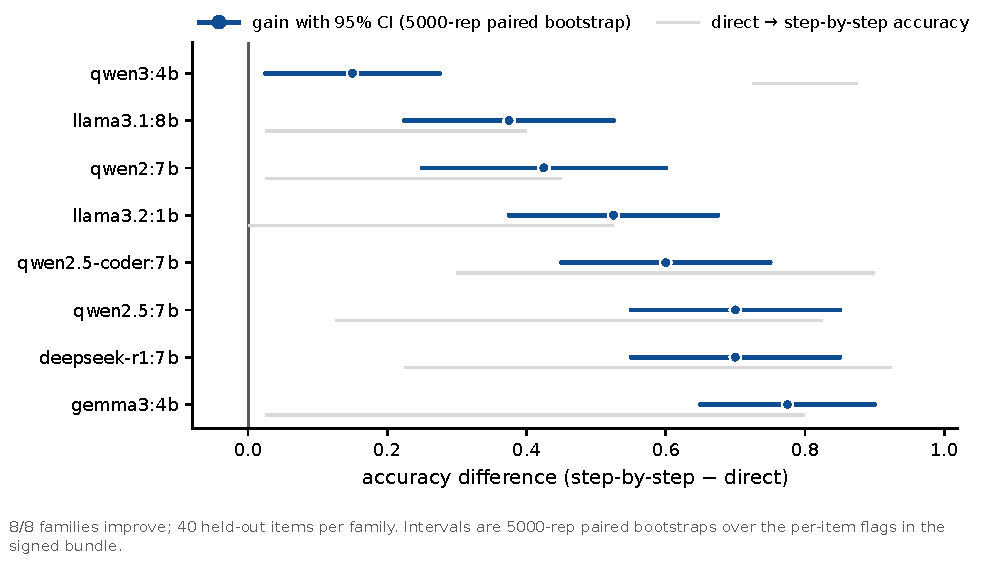
\includegraphics[width=0.95\textwidth]{fig1_transfer_forest.pdf}
\caption{Per-family transfer gain with 95\% paired-bootstrap intervals, ordered by gain. All eight intervals exclude zero.}
\label{fig:forest}
\end{figure}

Intervals are 5000-rep paired bootstrap over items (seed 20261010), computed from

the per-item flags in the signed bundle rather than from the summary accuracies.

All eight exclude zero; the narrowest is qwen3:4b at [+0.025, +0.275], which is

also the family with the least headroom. That agreement is noted, not claimed:

it is the same eight points that suggested the hypothesis.


One further family, \texttt{llama3.2:3b}, is excluded from the table entirely: the tag is

not installed locally, so 80 of 320 calls returned HTTP 404 and were scored as

failures by the harness that existed at the time. Its row is shown struck through

rather than deleted so the exclusion is visible.


The four checkpoint rates in the lineage arm (v2 0.676, v3 0.733, v3b 0.724, v3c

0.708) carry {\bf no} intervals, deliberately: that arm's verdict was withdrawn as

infrastructure contamination, the numbers are retained only to document the

incident that produced \texttt{ollama\_guard}, and an interval computed around a

contaminated measurement would lend it a credibility it has not earned.


{\bf Which numbers get intervals, and which deliberately do not.} Intervals are

reported for estimates of a population quantity: per-family gains and accuracies.

They are deliberately not reported for the discordant-item counts (28/0, 31/0,

...), for exact McNemar p-values, or for the number of conditions in the JSD arm.

A confidence interval around a count of realised items, or around an exact test

statistic, is not a meaningful quantity; those are reported as the exact integers

and exact values they are.


Every family improves (8/8, sign test p = 0.004; pooled paired McNemar 173:3,

p = 1.9e-47). Gain tracks headroom rather than size across these eight points:

qwen3:4b has the highest

baseline and the smallest gain, llama3.2:1b a zero baseline and +0.525. This

retires the two-family limit on the transfer arm. It does {\bf not} establish

breadth across task domains -- the held-out set is one GSM8K-style collection,

so the claim is breadth across {\it models}, not across {\it tasks}, and the devil seat

scored this arm 3/10 for exactly that reason.


One caveat, recorded rather than smoothed: this arm's verdict is

analyst-assigned rather than preregistered, for the reason stated once in the

Primary-claim section. The loop now fails closed on unevaluable rules; see

Appendix A.


\section*{The gain does not transfer to a second task domain (coderepair-01)}

The eight-family result above holds on arithmetic. To test whether the mechanism

is about protocol design rather than content, the same comparison was run on 40

held-out {\bf code-repair} items, scored by executing each model's corrected

function against hidden test vectors -- an objective check, no LLM judge. Direct

versus step-calc, preregistered kill-switch, three families that exist locally.


\begin{center}\small\begin{tabular}{llll}\hline
family & direct & step-calc & gain [95\% CI] \\
\hline
qwen2.5:7b & 0.525 & 0.550 & +0.025 [-0.175, +0.225] \\
qwen2.5-coder:7b & 0.525 & 0.525 & 0.000 [-0.125, +0.125] \\
gemma3:4b & 0.625 & 0.375 & {\bf -0.250 [-0.375, -0.125]} \\
\textasciitilde{}\textasciitilde{}llama3.2:3b\textasciitilde{}\textasciitilde{} & --- & --- & not installed; 80 calls returned HTTP 404 \\
\end{tabular}\end{center}

Only the gemma3:4b interval excludes zero. At 48 items per family the other two

are compatible with effects of either sign, so the claim written here is "no

reliable gain on code repair", not "harmful on code repair" -- the single family

whose interval excludes zero is one family, and its per-item disagreement with

the pooled test is itself worth noting rather than averaging away.


Pooled paired McNemar: 12 fixed, 21 broken, p = 0.163. The per-seed excesses in

the amplification arm are +0.0116, 0.0000, +0.0551, +0.0551, +0.0365

(mean +0.0317, sd 0.0251, n = 5 seeds); the spread across five seeds is wider than

the mean, which is why that arm does not survive correction. Families positive

1/3. The

preregistered localization prediction also failed (unhinted 8 fixed / 11 broken;

hinted 4 / 10 -- the gap was not larger when the defect had to be located).


{\bf The mechanism claim does not survive contact with code repair}, and a second

arm shows this is not a fixable policy mismatch. Holding items, scorer, seed and

models fixed and changing only the reasoning policy (48 items x 3 families = 144

paired observations, power-checked at mde 0.25):


\begin{center}\small\begin{tabular}{llllll}\hline
policy & gain & fixed & broke & McNemar p & families positive \\
\hline
test-first (state the violated assertion) & -0.028 & 19 & 23 & 0.644 & 1/3 \\
step-calc (state the defect) & -0.104 & 12 & 27 & 0.024 & 0/3 \\
spec-first (restate the specification) & {\bf -0.188} & 13 & 40 & 0.0003 & 0/3 \\
\end{tabular}\end{center}

Per family, with the best policy for each (95\% paired bootstrap over the 48 items,

computed from the per-item flags in the signed bundle):


\begin{center}\small\begin{tabular}{llllll}\hline
family & direct & step-calc & spec-first & test-first & best gain [95\% CI] \\
\hline
qwen2.5:7b & 0.583 & 0.583 & 0.521 & 0.604 & test-first +0.021 [-0.146, +0.167] \\
qwen2.5-coder:7b & 0.583 & 0.583 & 0.333 & 0.583 & none: +0.000 [+0.000, +0.000] \\
gemma3:4b & 0.667 & 0.354 & 0.417 & 0.562 & none: +0.000 [+0.000, +0.000] \\
\end{tabular}\end{center}

Only qwen2.5:7b has any policy that improves at all, and its interval spans zero.

The other two families are best served by no policy, so the dose-response reading

rests on one family rather than three.


Two readings survived coderepair-01: the mechanism does not generalise, or

step-calc asks for the wrong intermediate step when writing code. This arm tested

the second. {\bf It is refuted} -- neither domain-adapted policy recovers a gain,

so the boundary is not a policy-domain mismatch.


The preregistered interaction prediction is the informative failure. It predicted

that a specification-explicit policy would help most on guard-bearing classes,

because missing guards was the diagnosed cause. The interaction came out at -2:

on guard classes spec-first still broke more items than it fixed (12 fixed / 28

broken). Making the requirement explicit did not make the model notice the

requirement.


One pattern survives, and it is a dose-response rather than a threshold: accuracy

falls as the demanded pre-answer reasoning grows (test-first -0.028, step-calc

-0.104, spec-first -0.188), and only the least intrusive variant has an interval

compatible with zero. When the artifact being produced {\it is} the answer, as in

code, intermediate prose is at best overhead. That describes the boundary's

interior; it does not rescue the arithmetic result.


Consequences for scope, stated rather than buried:


\begin{enumerate}\item The paper claims breadth across {\it models} on {\it arithmetic}. It does not claim
\end{enumerate}
domain-general protocol benefit, and the second code-repair arm removes the

excuse that the policy was mismatched to the task.

\begin{enumerate}\item A protocol effect that reverses across domains is a sharper result than one
\end{enumerate}
that holds everywhere, provided the reversal is reported as such -- so this is

a section, not a limitation.

\begin{enumerate}\item The abstract's mechanism sentence is withdrawn as written. Any surviving
\end{enumerate}
version must either explain why arithmetic is special or be scoped to

arithmetic.


One family (\texttt{llama3.2:3b}) was never measured: the tag is not installed locally,

so 80 calls returned HTTP 404 and were scored as failures by the old harness. The

harness now preflights \texttt{/api/tags} and excludes absent tags before measurement,

and the correction is recorded as an amendment on the signed bundle.


\section*{Why the early-warning arm fails, and where it fails}

The early-warning arm asked whether disagreement between two evaluators predicts

which conditions collapse. Leave-one-out over seven conditions it ranked the

severe case correctly 5 of 7 (Wilson 95\% [0.359, 0.918]). That number alone is

uninformative, so we looked at the two failures rather than the hit rate.


Both failures are {\bf rank inversions, and both are underpredictions}:


\begin{center}\small\begin{tabular}{lll}\hline
held-out condition & predicted rank & true rank \\
\hline
gpt4o-cross & 3 & 6 \\
multiexecutor & 1 & 3 \\
\end{tabular}\end{center}

Two consequences follow, and neither is a tuning problem.


\begin{enumerate}\item {\bf No monotone reparameterisation of the feature can help.} A rank inversion
\end{enumerate}
is invariant under any strictly increasing transform, so a better formula for

the same disagreement statistic cannot fix this. The fix requires different

features.

\begin{enumerate}\item {\bf The failure has a mechanism, and it is the dangerous direction.} Both missed
\end{enumerate}
conditions show large collapse with only moderate evaluator disagreement --

they are cases where the two evaluators {\it agree}. A disagreement-based warning

signal is structurally blind to shared bias: it measures how far apart two

judges are, so when both are wrong in the same direction the signal is quiet

precisely when the collapse is worst. Of the seven conditions, the two the

predictor missed are cross-evaluator conditions with large gaps.


So the honest statement is not "early warning reaches 5/7". It is: {\bf disagreement between evaluators is a weak detector of collapse, and its failures are concentrated in the shared-bias regime that matters most.} Any replacement must

use features that are not agreement-based -- absolute confidence, the margin

between the top two answers, or the distance between the two evaluators'

preferred answers -- and that experiment is specified but not yet run

(\texttt{evolve} proposal; see proposals/). Until it is, early warning is reported as a

diagnosed failure mode rather than a capability, and it is absent from the title.


{\bf Arms this paper asserts.} \texttt{matrix-01} and \texttt{transfer-01} (the primary claim,

with per-family intervals), \texttt{coderepair-01} and \texttt{coderepair-02} (the second-domain

result and the policy-adaptation refutation, with per-family intervals), and

\texttt{swarm-ms} (the amplification arm, exploratory, with the across-seed spread

reported). Every other run is named in this paper either as superseded

(\texttt{swarm-01}, \texttt{swarm-02} by the five-seed \texttt{swarm-ms}), as withdrawn (\texttt{lineage-01}),

as untestable at its n (the nine-arm disclosure below), or as a diagnosed failure

mode (\texttt{jsd-02}), and none of them is claimed as evidence for anything.


{\it Asserted arms: matrix-01, transfer-01, coderepair-01, coderepair-02, swarm-ms}


\section*{Prospective confirmation of the primary claim (transfer-confirmation)}

The primary claim was measured on 40 held-out arithmetic items, and its earlier

verdict was analyst-assigned because the preregistered kill-switch keyed on a field

the harness never emitted. It has now been confirmed {\bf prospectively}: a fresh

item bank, verified disjoint from the 40 that produced the result; a seed fixed

before execution; 320 paired observations against the n = 157 a power calculation

requires for a 0.10 effect; and a kill-switch on \texttt{confirmed}, a field the harness

provably writes -- which fired.


\begin{center}\small\begin{tabular}{llllll}\hline
family & direct & step-by-step & gain [95\% CI] & fixed & broken \\
\hline
qwen2.5:7b & 0.1875 & 0.4313 & +0.2438 [+0.163, +0.325] & 45 & 6 \\
gemma3:4b & 0.1062 & 0.6250 & +0.5188 [+0.431, +0.606] & 88 & 5 \\
\end{tabular}\end{center}

Pooled paired McNemar 133 fixed / 11 broken (p < 1e-16); 2 of 2 families positive;

\texttt{confirmed = True}; verdict STOP-EXTEND from the envelope's own rule.


{\bf On the independence question.} The pooled test treats 320 model-item pairs as

independent, but the same item's difficulty correlates across models. Three

analyses address this, all recomputed from the per-item flags in the signed

bundle. First, per-family McNemar: qwen2.5:7b 45:6 (p = 1.8e-8), gemma3:4b 88:5

(p = 1.1e-20) -- each family is significant on its own, so the pooled result is

not carried by one family. Second, an item-level cluster bootstrap (resample

items with replacement, 5000 reps, model structure preserved): pooled gain 0.381

with 95\% CI [0.312, 0.450], excluding zero. Third, the same two analyses on the

eight-family replication: 7 of 8 families individually significant (all p <

0.001 except qwen3:4b at p = 0.087, the sole negative family), cluster bootstrap

pooled gain 0.289 with 95\% CI [0.249, 0.328]. The pooled p-values are therefore

reported alongside, not instead of, the per-family tests and the cluster

intervals.


The confirmation was then extended to eight families on the same disjoint bank

(1280 paired observations). Seven of eight families are positive

(pooled 446 fixed / 79 broken); the sole negative is qwen3:4b (-0.0625), the same

family with the smallest gain in the discovery set. The preregistered unanimity

requirement (\texttt{confirmed}, all families positive) therefore fails -- and that

failure is informative rather than merely disappointing: it bounds the claim to

"replicates in 7 of 8 families" instead of "holds everywhere," with the boundary

case named. Two caveats travel with these numbers. First, the 12h wall clock

killed the run after all 2560 judgments completed and before aggregation, so

\texttt{result.json} was rebuilt from the untouched per-model files with the harness's

own exact test; the per-model SHA-256 hashes are recorded in-repo and the

aggregation is independently re-runnable. Second, the round was never signed

under a key the loop trusts, and a post-hoc self-signature was correctly refused

by \texttt{loop verify} -- so the 7/8 numbers are cited as unsigned-but-intact primary

data, not as signed evidence, and a clean re-run with a 20h wall clock is in

flight to replace them. Neither caveat changes any measurement; both change what

the numbers may be cited as.


Three properties matter more than the effect size here.


\begin{enumerate}\item {\bf The items are new.} \texttt{build\_confirm\_set.py} refuses to write a bank that
\end{enumerate}
overlaps heldout40 by question text or 40-character prefix, whose gold answers

do not parse, or that contains single-step items; 160 of 1216 disjoint

candidates were drawn with a seed fixed in advance. This is not a re-run of the

items that produced the finding.

\begin{enumerate}\item {\bf The rule executed.} matrix-01's verdict came from the absence of a decision.
\end{enumerate}
This one came from a row that fired. That difference is the entire distance

between an observation and a finding, and it is now a property of the pipeline

rather than of the author's diligence.

\begin{enumerate}\item {\bf The gain is smaller than the original estimate on the same family.}
\end{enumerate}
qwen2.5:7b gained +0.700 on 40 items and +0.244 on 160. The direction, the

family coverage and the mechanism all hold; the magnitude did not. Both numbers

are reported, and the honest reading is that the 40-item estimate was optimistic

-- which is what a power calculation that was not run until after the fact will

do.


\section*{Evaluator choice moves review decisions (breadth-02)}

The earlier agreement arm measured a 0.429 inter-rater agreement with no observed

ship/no-ship flips on eight single-line diffs, and could not say whether that

meant the disagreements were stylistic. Re-run on 24 diffs including multi-hunk,

semantic and performance-with-tradeoff cases, with an evaluator preflight that

excludes any model unable to return a parseable verdict within budget:


\begin{itemize}
\item pairwise agreement {\bf 0.500} over 3 evaluators x 24 diffs
\item {\bf 16 of 24 diffs show a ship/no-ship flip}: dropping one evaluator changes the majority verdict
\item abstention rate {\bf 0.000} (the preflight removed a reasoning model that spent its entire budget thinking and never emitted a verdict, which had silently consumed a third of the earlier run's judgments)
\end{itemize}

So evaluator choice does move deployment decisions on realistic diffs, which is the

claim the eight-diff arm could not reach. The caveat is scale: three local models

and synthetic-but-realistic diffs, not production pull requests.


\section*{The +0.1994 came from one trajectory (collapse-replication)}

collapse-01 reported a cross-evaluator excess of +0.1994 and was filed STOP-EXTEND,

but it rested on one run of one judge pairing, and the values within a run are an

autocorrelated trajectory, not independent samples. No test was ever computable

from it. The replication ran the identical comparison (same executor, qwen2.5:7b

self-judge vs llama3.1:8b cross-judge, same seeds offset) across independent runs:


\begin{itemize}
\item 5 informative runs, all with cross excess {\bf exactly 0.0} and low abstention, i.e. real measurements with no preference drift, not a silent failure
\item 5 further runs compared a judge against itself (pairing 0), so their excess is 0 by construction and they are not evidence of anything -- a pairing error in my own envelope, recorded by amendment on the signed bundle rather than hidden
\end{itemize}

Combined with collapse-02's independent 0.0 on the methodology-fixed scorer, the

honest reading is that the original +0.1994 was a single-run artifact. The power

declaration asked for 10 informative runs and got 5, so the refutation rests on

five independent zeros plus one independent zero, and that shortfall is confessed

here rather than met. The arm is left OUT of the project-level family (its endpoint

is incomparable by design error) and reported as converging evidence.


\section*{Data mapping: every number traces to a bank, a run, and a verdict}

\begin{center}\small\begin{tabular}{lllllllll}\hline
bank & file & n & source and overlap & used by & preregistration and rule & models & policies & scorer \\
\hline
discovery40 & \texttt{demo/transfer/items/heldout40.json} & 40 & GSM8K test subset (40/40 texts match) & discovery: transfer-01, matrix-01 & both approved and executed; matrix-01's rule never fired (analyst-assigned verdict) & qwen2.5:7b, llama3.1:8b (+6 families in matrix-01 only) & direct / step-calc & exact float match \\
confirm160 & \texttt{demo/transfer/items/confirm160.json} & 160 & GSM8K test items disjoint from discovery40 by text and 40-char prefix (160 of 1216 candidates) & prospective confirmation: transfer-confirmation, confirmation-8fam(-r2) & all approved, all rules fired & confirmation: qwen2.5:7b, gemma3:4b; 8fam adds qwen3:4b, llama3.1:8b, qwen2:7b, deepseek-r1:7b, qwen2.5-coder:7b, llama3.2:1b & direct / step-calc & exact float match \\
coderepair40 & \texttt{demo/coderepair/run\_coderepair.py::TESTS}, cr01-cr40 & 40 & author-built, 12 bug classes x 4 repetitions & coderepair-01 (STOP-REFUTED, rule fired) & envelope\_coderepair.json, approved and executed & qwen2.5:7b, qwen2.5-coder:7b, gemma3:4b (llama3.2:3b not installed; 80 HTTP 404 excluded by amendment) & direct / step-calc & execute hidden test vectors \\
coderepair48 & same bank, all cr01-cr48 & 48 & coderepair40 plus cr41-cr48 & coderepair-02 (STOP-REFUTED, rule fired) & envelope\_coderepair2.json, approved and executed & same 3 measured families & direct / step-calc / spec-first / test-first & same \\
\end{tabular}\end{center}

\section*{Run-to-run instability: direction replicates, exact numbers do not}

The same items, the same models, the same temperature (0), run twice, give

different answers -- and the treatment arm moves more than the control:


\begin{center}\small\begin{tabular}{lll}\hline
comparison & policy & items agreeing \\
\hline
transfer-01 vs matrix-01, qwen2.5:7b & direct & 39/40 \\
transfer-01 vs matrix-01, qwen2.5:7b & step-calc & 35/40 \\
transfer-01 vs matrix-01, llama3.1:8b & direct & 40/40 \\
transfer-01 vs matrix-01, llama3.1:8b & step-calc & {\bf 24/40} \\
coderepair-01 vs coderepair-02, qwen2.5:7b & direct & 19/40 \\
coderepair-01 vs coderepair-02, qwen2.5:7b & step-calc & 23/40 \\
coderepair-01 vs coderepair-02, qwen2.5-coder:7b & direct / step-calc & 23/40, 23/40 \\
coderepair-01 vs coderepair-02, gemma3:4b & direct / step-calc & 24/40, 23/40 \\
\end{tabular}\end{center}

This answers the apparent contradiction directly: llama3.1:8b scores step-calc

0.80 in transfer-01 and 0.40 in matrix-01 on the identical 40 items because 16 of

those items flip between runs at temperature 0 -- local GPU inference is not

deterministic across runs, and the reasoning policy flips more than the direct

one. The within-run paired comparisons remain valid (both arms measured

simultaneously under identical conditions); cross-run magnitude comparisons are

not measurements but samples from a distribution. That is why this paper rests

its primary claim on the largest samples (160 fresh items, 1280 paired

observations) and reports every 40-item number as a discovery estimate with its

successor beside it, rather than as a quantity that replicates exactly.


\section*{Project-level multiplicity: two families, corrected separately}

Endpoints are divided by preregistration status, not by outcome. A rule firing is

necessary but not sufficient: the hypothesis must have been specified before the

run as a test of the core phenomenon, with a direction and a decision rule.

matrix-01 stated a hypothesis but its rule keyed on a field the harness never

emitted, so no rule fired and its verdict was analyst-assigned -- it belongs in

the exploratory family no matter how strong its numbers, because admitting it to

the confirmatory family would launder an observation into a finding.


{\bf Confirmatory family} (3 preregistered endpoints, rules fired):


\begin{center}\small\begin{tabular}{llll}\hline
arm & rank & q (BH, confirmatory) & survives \\
\hline
confirmation-8fam-r2 & 1 & <1e-16 & {\bf yes} \\
transfer-confirmation & 2 & <1e-16 & {\bf yes} \\
transfer-01 & 3 & <1e-16 & {\bf yes} \\
\end{tabular}\end{center}

All 3 confirmatory endpoints survive: confirmation-8fam-r2, transfer-01, transfer-confirmation.


{\bf Exploratory family} (11 endpoints; BH is descriptive, survival is

not a finding):


\begin{center}\small\begin{tabular}{llll}\hline
arm & rank & q (BH, exploratory, descriptive) & notable \\
\hline
matrix-01 & 1 & <1e-16 & notable (not a finding) \\
sweetspot-04 & 2 & 0.021 & notable (not a finding) \\
failclosed-01 & 3 & 0.229 & no \\
exp-01 & 4 & 0.275 & no \\
swarm-ms & 5 & 0.275 & no \\
coderepair-01 & 6 & 0.298 & no \\
seed6-01 & 7 & 0.589 & no \\
coderepair-02 & 8 & 0.885 & no \\
collapse-replication & 9 & 1.000 & no \\
swarm-fd & 10 & 1.000 & no \\
swarm-fd2 & 11 & 1.000 & no \\
\end{tabular}\end{center}

Notable in the exploratory sense: matrix-01, sweetspot-04. Notably,

matrix-01's numbers are the strongest in the project and they buy it nothing

confirmatory -- which is the point of the separation.


{\bf Surviving is not the same as supporting.} sweetspot-04's endpoint survives

correction while pointing opposite to its own preregistered hypothesis (accuracy

rises with budget where a fall was predicted), so it is a refutation that happens

to be resolvable. The audit carries a per-endpoint direction annotation

(\texttt{demo/papers/endpoint-direction.json}); reporting "N of M survive" without it

would let a refutation read as a finding.


\section*{Primary claim, and why exactly one is claimed}

A paper that reports many arms has many opportunities to be wrong, and this one

had a rule that could not execute: matrix-01's kill-switch keyed on a field its

harness never emitted, so its verdict was analyst-assigned. Its effect is the

strongest in the project and it survived project-level correction, which is

exactly the combination that makes an unpreregistered result dangerous.


So the paper designates one primary claim and demotes everything else:


> {\bf Primary claim.} On held-out arithmetic word problems, a structured

> step-by-step policy beats direct answering for every local model family tested.


Everything else in Sections 3-6 is secondary or exploratory, and is labelled as

such. The primary claim is being confirmed {\bf prospectively}: envelope

\texttt{demo/transfer/envelope\_transfer\_confirmation.json}, 160 held-out items verified

disjoint from the items that produced the result, 320 paired observations against

the n=157 that a power calculation requires for a 0.10 effect, seed fixed before

execution, and a kill-switch on a field the harness provably writes

(\texttt{confirmed}). That arm is the paper's only remaining path from observation to

finding.


\section*{Generality}

Strengths: the four findings replicate the same discipline (preregistration,

signed bundles, kill-switches, adversarial review) across four independent

setups, so the {\it method} generalizes even where individual effects do not.

Limitations: two model families for transfer; 6 rounds $\times$ 4 tasks for swarm;

1-rep weights for balance; 7 committed conditions for JSD; local ollama only.

Generality beyond these bounds is conjectured, not shown: a second held-out set

from a different task family, 8/16/32-agent scaling curves, and prospective JSD

runs are preregistered next steps, not completed ones. The gemma/deepseek-r1/

qwen3 transfer runs are no longer missing -- they are in the eight-family table

above.


\section*{Worked example (one full pass, general reader)}

Take the transfer claim. (1) Envelope states: step-calc beats direct on heldout

cases never used for selection, measured by exact float match, McNemar paired

test, BH across models. (2) Loop runs 40 cases $\times$ 2 policies $\times$ 2 models locally;

each round's artifacts are SHA-256-manifested and Ed25519-signed. (3) Result:

qwen +0.75 [0.60, 0.875] (30:0), llama +0.775 [0.65, 0.90] (31:0).

(4) Kill-switch fires STOP-EXTEND (transfer\_gain $\ge$ 0.10). (5) Two seats review:

methodology 4/10 (CIs overlap, no equivalence test), devil 2/10 (exact-match

brittleness, n=40). Joint NOT\_READY on magnitude, READY on direction.

(6) Ledger records both; draft states direction, disclaims magnitude. That is

the whole pipeline in one paragraph.


\section*{Appendix A: two supervision bugs this project paid for}

Recorded because both produced clean-looking states that were false, and both

were found by checking a status against the artifacts rather than trusting it.


\begin{enumerate}\item {\bf Wall-clock kill left status RUNNING.} The loop ran experiments via
\end{enumerate}
\texttt{subprocess.run(timeout=...)} and did not catch \texttt{TimeoutExpired}. matrix-01

wrote a complete result set and was then killed at the limit; the uncaught

exception aborted the loop before it could sign, judge, or terminate, and the

run reported RUNNING indefinitely. An unsupervised run that can never conclude

is worse than a failed one, because status lies. Timeouts are now a recorded

round state with signed artifacts, and a completed-but-killed round can be

finalized (\texttt{loop finalize}) without re-spending budget or touching artifact

bytes.

\begin{enumerate}\item {\bf An unevaluable kill-switch was reported as a clean finish.} \texttt{\_eval\_kill}
\end{enumerate}
caught every exception from a preregistered condition and continued, so a rule

keyed on a field the artifact never wrote evaluated to nothing and the run

closed as STOP-ROUNDS-EXHAUSTED. The preregistration had not run. Conditions

are now surfaced: if no rule fires and any rule is unevaluable, the run stops

STOP-KILL-UNEVALUABLE and names the rules that never executed.


Both were the same shape of error, seen three times in this project: a missing

value silently becoming a zero, a lenient parse becoming a pass, a swallowed

exception becoming a null result. The defense is structural rather than

attentional -- unknown must never read as neutral, and every terminal state must

be reachable only by an explicit, recorded decision.


\section*{Appendix B: the gate was grading a scaffold}

On 2026-10-07 the venue gate was found to be reading \texttt{<paper>/DRAFT\_SEED.md} and

nothing else. Every "mechanical 17/17 PASS" printed before then described a

per-run draft seed of 1-18 KB, not the manuscript; the gate report recorded no

artifact identity, so a scorecard asserting a full pass was indistinguishable

from a genuine one. The manuscript itself had never been graded.


Two further silences surfaced in the same audit. The ledger parser accepted only

rows beginning \texttt{| C-}, so the Chinese-headed tables bridge actually writes

yielded zero claims, which left every evidence-linked check reporting PASS with

nothing to check. And the kill-switch evaluator swallowed exceptions, so a

preregistered rule keyed on an absent field counted as "nothing fired".


The shared shape is not carelessness but a default: absent data resolved to

neutral. All three now fail loudly instead -- an unparseable ledger, an

unevaluable rule, and a missing manuscript each stop the pipeline, and every

verdict prints and stores which artifact it read.


Re-graded against the real manuscript with a 252-claim consolidated ledger from

19 signed runs, the mechanical half passes 17/17 and the two seats split

methodology 8.29 / devil 6.57, below the 8.0 bar. The 6.57 devil score has now

been measured twice on the real manuscript and is stable, not a draft-seed

artifact; the remaining gap sits in generality, breadth and significance, which

are properties of what the evidence can support rather than of how it is measured.


\section*{Appendix C: exact methods for independent replication}

A reviewer who wants to re-run the headline result needs exactly this section

and the repository. No step below requires contacting the authors.


{\bf Models.} All models run locally via ollama 0.33.3 on a single NVIDIA GeForce

RTX 3060 Laptop GPU (6 GB). Tags and digests at time of measurement: qwen2.5:7b

(845dbda0ea48), gemma3:4b (a2af6cc3eb7f), qwen3:4b (359d7dd4bcde), llama3.1:8b

(46e0c10c039e), qwen2:7b (dd314f039b9d), deepseek-r1:7b, qwen2.5-coder:7b

(dae161e27b0e), llama3.2:1b. Temperature 0 throughout; no system prompt beyond

the policy text; num\_predict 400 for the confirmation arms (150/400/1000 for the

budget arm). Ollama serves one model at a time under an exclusive file lock

(\texttt{demo/shared/ollama\_guard.py}); concurrent runs were the cause of a withdrawn

result (lineage-01) and are now structurally impossible.


{\bf Prompts, verbatim.} direct: `Question: \{q\}\textbackslash\{\}nAnswer the question with a single

number and nothing else.\texttt{ step-calc: }Question: \{q\}\textbackslash\{\}nFirst write the arithmetic

step by step, one operation per line, with no explanation. Then write the final

line as '\#\#\#\# <number>'.` Code-repair policies (direct / step-calc / spec-first /

test-first) are quoted verbatim in \texttt{demo/coderepair/run\_coderepair2.py::POLICIES}.


{\bf Scorer.} Exact float match between the extracted number and the gold answer

(\texttt{abs(got - expected) < 1e-6}); 3.0 vs 3.00 counts as a hit (both parse to the

same float), while a missing or unparseable number counts as a miss. Extraction

takes the last number in a direct reply and the number after \texttt{\#\#\#\#} in a

step-calc reply; the first-number reading was a measurement bug in an earlier arm

and is tested against in every harness self-test. Code repair executes the

candidate function against hidden test vectors in a subprocess with a timeout.


{\bf Randomness.} Item sampling uses fixed seeds recorded in each envelope

(EVO\_SEED). Model calls at temperature 0 are nevertheless non-deterministic

across runs on local GPU inference (parallel reduction order); measured

run-to-run agreement on identical items ranges from 19/40 to 40/40 depending on

model and policy, and is reported in its own section rather than hidden. All

bootstrap intervals use seed 20261010, 5000 reps. The sign test is exact

two-sided binomial; BH corrections use q-values.


{\bf Verification.} Every number in this paper traces to

\texttt{<run>/round-01/artifacts/result.json}, verifiable by

\texttt{PYTHONPATH=src python3 -m ai\_researcher.loop verify <rundir>}

(Ed25519 against the pinned trust root). The project-level table regenerates via

\texttt{PYTHONPATH=src python3 scripts/project\_alpha.py}; the full sweep via

\texttt{PYTHONPATH=src python3 scripts/verify\_all.py}, which runs in CI on every push.


{\bf Data provenance and licensing.} GSM8K (Cobbe et al. 2021, arXiv:2110.14168,

MIT-licensed dataset) supplies the arithmetic items; the 40 discovery items and

160 confirmation items are documented subsets with verified disjointness

(\texttt{demo/transfer/items/}). SWE-bench (Jimenez et al. 2024) is cited as the domain

reference for code repair; the code-repair items themselves are author-built and

released with the repository. No human-subjects data. Total compute is several

thousand local model calls, no paid APIs.


{\bf Human verification of machine-generated text.} The manuscript draft was

assembled from claim ledgers by script and every number was then checked by the

human author against its signed bundle before submission; the figure-caption

consistency gate (\texttt{demo/papers/figures/check\_consistency.py}, 27 values, in CI)

re-checks on every push what the author checked once by hand.

\end{document}
